%!TEX root = ../main.tex
%chktex-file 36

\chapter{The Current State of Gillian}\label{sec:current}

The continuation of work on Gillian and its debugger requires a deep
understanding of their driving principles and implementation details.
These aspects, as well as their shortcomings in the current state of Gillian,
are outlined here.

\section{Symbolic Execution with Unification}\label{sec:current:symex}

\todo{Describe SybmEx in more detail?}

While symbolic execution is an essential component of program verification, it
alone is not sufficient for applying separation logic when reasoning about a
program. The `gotcha' step that bridges symbolic exection to separation logic is
the process of \textbf{unification}, where a symbolic state is matched against a
particular condition in separation logic. Gillian does this by transforming the
relevant condition into a \textbf{unification plan} (or \textbf{UP}), where each
step is an assertion that the current state must be matched against, potentially
after finding appropriate substitutions.

It's worth noting that Gillian has a notion of a \textit{predicate state} in
addition to symbolic state, where the former is an extension of the latter that
includes predicates. This becomes integral to the unification process when
considering logic that contain predicates, as predicates can be defined
recursively, and thus cannot be considered in pure separation logic. This way,
the act of building a predicate from its component parts (in practice, unifying
the state against the definition of the predicate) can be delegated to a
subproblem, dubbed \textbf{folding}.

\begin{lstlisting}[caption={
  The recursive list length function, in WISL
  \label{lst:llen-rec}}, style=code]
  { (x == #x) * list(#x, #alpha) }
  function llen(x) {
      if (x = null) {
          n := 0
      } else {
          t := [x+1];
          n := llen(t);
          n := n + 1
      };
      return n
  }
  { list(#x, #alpha) * (ret == len(#alpha)) }
\end{lstlisting}

\begin{figure}
  \center{}
  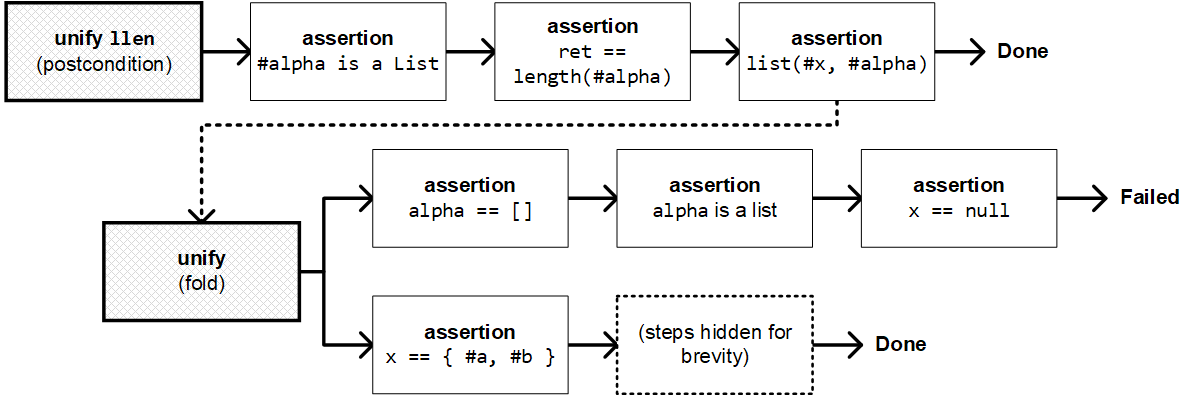
\includegraphics[width=0.8\textwidth]{img/unify-example.png}
  \caption{
    An example of unification --- the postcondition of \texttt{llen}'s non-empty
    case --- including a fold}\label{fig:unify-example}
\end{figure}

\autoref{fig:unify-example} outlines the process of unifying the recursive list
length function, \texttt{llen} (\autoref{lst:llen-rec}), which makes use of the
\texttt{list} predicate (see \autoref{lst:list-predicate}). The top-level
unification plan comprises of:
\begin{itemize}
  \item Assert that the logical variable \texttt{\#alpha} is a list
  \item Assert that the program variable \texttt{ret} is set to the list of
        \texttt{\#alpha}
  \item Assert that the program variable \texttt{x} points to a linked list,
        whose contents are equal to \texttt{\#alpha}
\end{itemize}
The first two assertions are readily available in the predicate state, however
the final assertion has no direct match; the only instance of the \texttt{list}
predicate in our state is for the tail of the given list. Therefore, since
Gillian is attempting to unify a predicate assertion, it attempts a fold.
Here, two different unifications are considered; one for the \texttt{list}
predicate's empty case, and one for its non-empty case. The empty case
unification fails; this is trivially true, as in \texttt{llen}'s non-empty case,
\texttt{x} cannot be \texttt{null}. The remaining unification, after a number of
assertions that build up the \texttt{list} predicate's non-empty case,
eventually succeeds, proving that \texttt{list(\#x, \#alpha)} holds for this
predicate state. As that was the final top-level assertion, the overall
unification has now succeeded.

This process of unification is one of the core pillars of Gillian's
functionality, yet it remained unrepresented by the debugger available prior to
this project.


\section{The Gillian Interpreter}\label{sec:current:interpreter}

Taking a single symbolic execution step in Gillian's interpreter follows
the general process of:
\begin{itemize}
  \item Pop the first symbolic state configuration from the stack. If the stack
        is empty, then execution has finished, and the execution result is
        returned.
  \item Perform the action required by that configuration --- usually executing
        the next command in the program.
  \item Push any new state configurations to the stack. There can be multiple
        new states, for example, when symbolic execution branches at an if/else
        statement.
\end{itemize}

In previous work, this process was extended to not simply perform symbolic
execution to completion immediately, but instead, provide a continuation
function (\texttt{cont\_func}; see \autoref{lst:contfunc-type-original}) ---
essentially a thunk that, once called, executes a single symbolic execution
step, returning the result of that step, and a new \texttt{cont\_func} to
execute the next one; the original behaviour of running to completion can be
recreated by repeatedly executing the given thunks until the \texttt{Finished}
case is returned.

\begin{lstlisting}[caption={
  The original \texttt{cont\_func} type
  \label{lst:contfunc-type-original}}, style=code, numbers=none]
  type 'a cont_func =
  | Finished of 'a list
  | Continue of (cconf_t list * (unit -> 'a cont_func))
\end{lstlisting}

While this meets the basic needs of step-by-step execution for a debugger, it
proves to be a fairly blunt instrument, giving minimal information to the
debugging process, and no control outside of when to execute the next step.


\section{Symbolic Trace and the Logging Structure}\label{sec:current:trace}

Originally, the log reports made to a file were the only way to debug
verification. This changed when, in a previous project, Radu Lacraru
~\cite{gillian-logging-2020} provided mechanisms for making more detailed
reports to an SQLite database for later querying. While this opens the door for
more structured logging, and a trace that more closely matches Gillian's
symbolic execution and unification processes, this is not used to its fullest
potential in the current debugging implementation.

\begin{lstlisting}[caption={
  The \texttt{Report.t} type
  \label{lst:report-type}}, style=code, numbers=none]
  (* report.ml *)

  type t = {
    id : ReportId.t;
    title : string;
    elapsed_time : float;
    previous : ReportId.t option;
    parent : ReportId.t option;
    content : Loggable.t;
    severity : severity;
    type_ : string;
  }
\end{lstlisting}

Of particular note is the \texttt{Report.t} type's (\autoref{lst:report-type})
\texttt{content} field, which is used to store various information in JSON
format, which can then be parsed straight back into the relevant data structure
and used when querying logs; the specific data structure stored is dictated by
the \texttt{type\_} field, which is set to one of a set of preset strings
(\autoref{lst:loggingconstants}).

While \texttt{Report.t} supports references to a \texttt{parent} and
\texttt{previous} report, these were not utilised in log querying whatsoever,
instead relying on the \texttt{elapsed\_time} field to deduce which reports
preceded and succeeded others. The current logging structure, shown in
\autoref{fig:log-structure-current}, is merely a consequence of when and where
in Gillian's code that logging was performed, rather than being backed by
principled decisions. Note that the `assertion' reports did not in fact exist
prior to this project, but are shown where they would be if added before log
restructuring.

\begin{sidewaysfigure}
  \center{}
  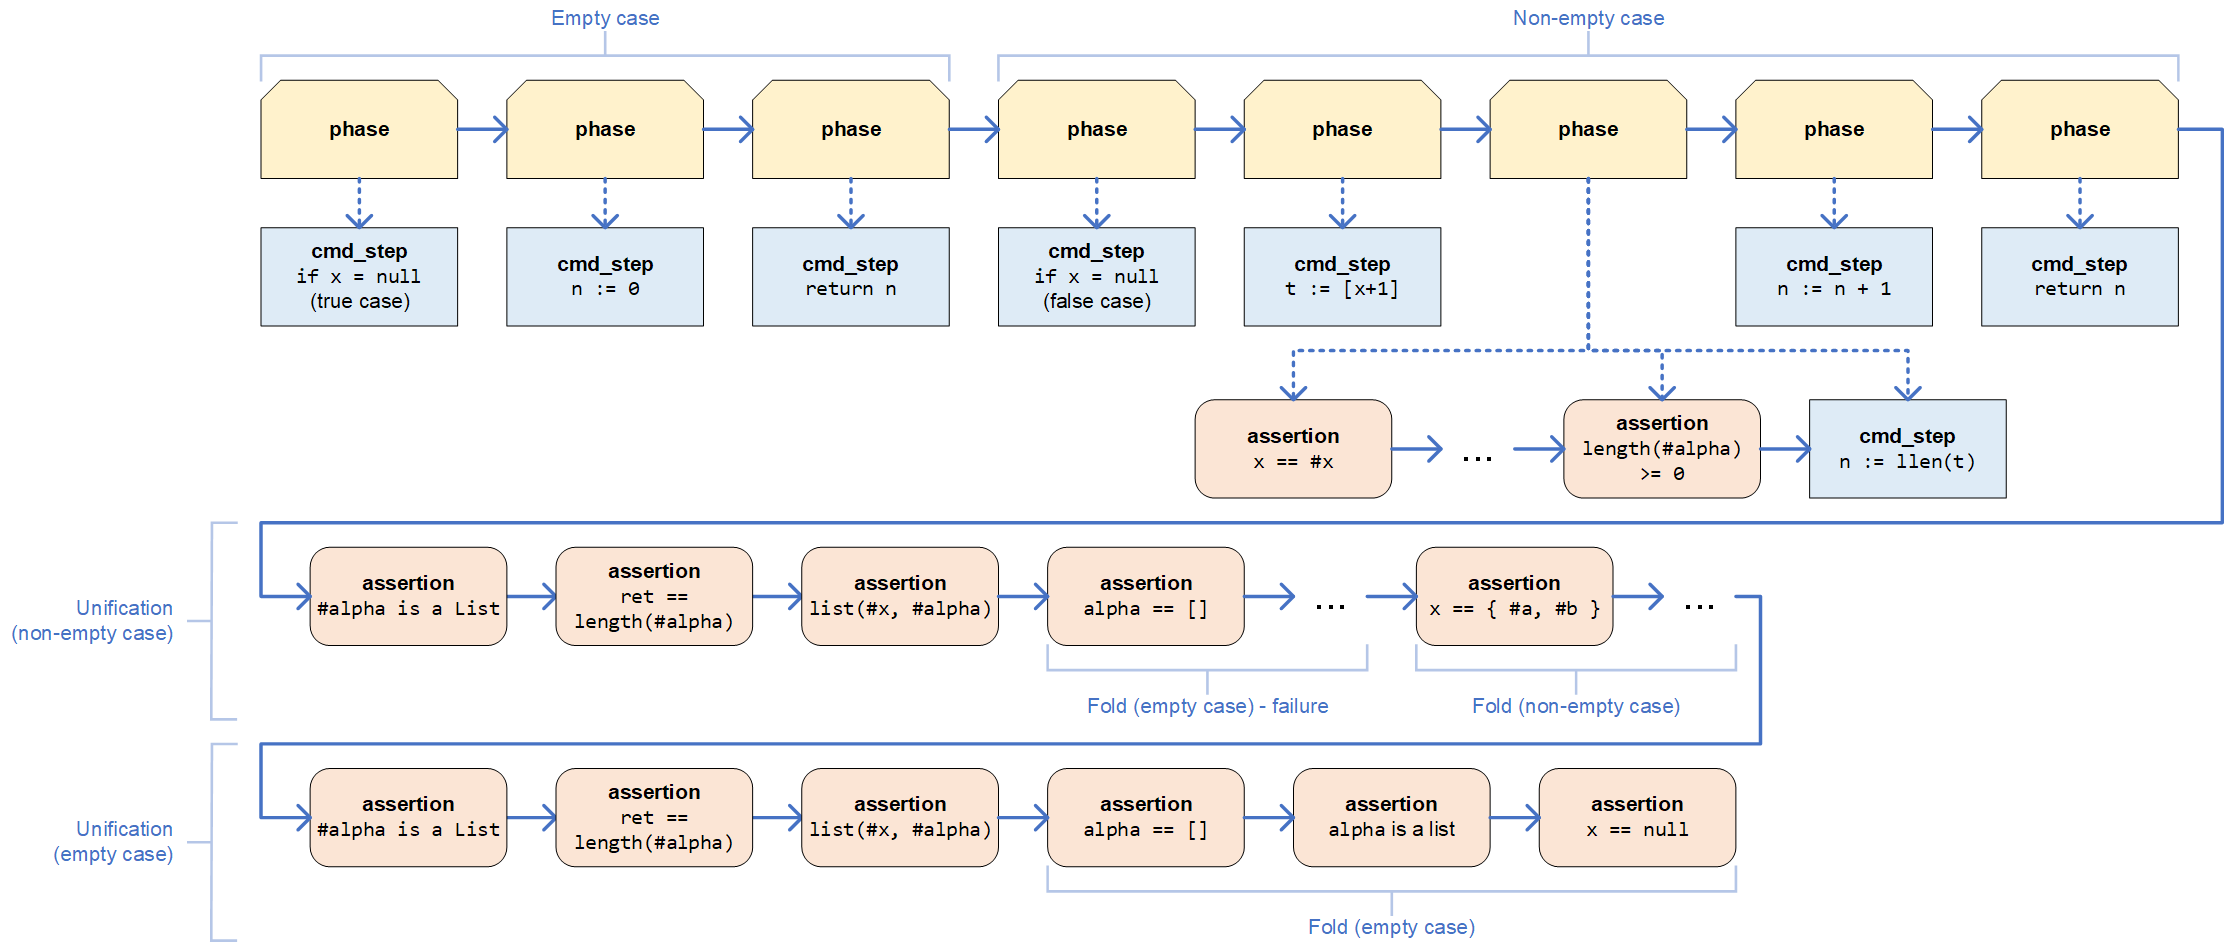
\includegraphics[width=0.95\textwidth]{img/log-structure-current.png}
  \caption{The original reporting structure for Gillian debugging, with added 
    `assertion' reports}\label{fig:log-structure-current}
\end{sidewaysfigure}

While the current logging structure is of no meaningful use, the logging
mechanisms provided serve as a very strong foundation for further improvements
to Gillian debugging.


\section{Debug Adapter}\label{sec:current:dap}
\todo{Write section}
